\documentclass[12pt]{article}
\usepackage[a4paper]{geometry}
\usepackage[utf8]{inputenc}
\usepackage{url}
\usepackage{hyperref}
\usepackage[french]{babel}
\usepackage[T1]{fontenc}
\usepackage{graphicx}
\usepackage{tgheros}
\usepackage{listings}
\usepackage{forest}
\renewcommand{\familydefault}{\sfdefault}

\lstset
{ 
    language=xml,
    basicstyle=\footnotesize,
    numbers=left,
    stepnumber=1,
    showstringspaces=false,
    tabsize=4,
    breaklines=true,
    breakatwhitespace=false,
}

\title{Rapport Projet Tuteuré Rundeck}
\author{HEPPNER Tristan / ROYER Grégory
\\
TORRES Yanis / AISSI Ayoub }
\date{Janvier 2020}

\begin{document}

\maketitle
\newpage
\tableofcontents
\newpage
\section{Remerciements}

Nous remercions notre tuteur de projet tutoré, Mr Fabien PASCALE, Expert en calcul scientifique au CNRS, pour nous avoir fait découvrir Rundeck, ses enjeux ainsi que l'ampleur et l'importance de ce projet.
\vspace{0.5cm}
\\
Merci  à  Monsieur Lucas  Nussbaum,  Debian  Project  Leader  (DPL),  maître  de conférences à l'Université de Lorraine et chercheur auprès du laboratoire LORIA, pour nous avoir permit de nous enrichir intellectuellement.
\vspace{0.5cm}
\\
Que cette licence ASRALL(Administration de Systèmes, Réseaux et Applications à base  de  Logiciels  Libres)  puisse  perdurer  dans  le  temps,  et  toujours  apporter  les connaissances indispensables dont nous, les élèves et futurs administrateurs, avons besoin. Un grand merci à Monsieur Philippe Dosch, enseignant et responsable de la licence, qui a su, quand il le fallait, nous écouter et nous donner les indications nous permettant de prendre la bonne direction.
\newpage
\section{Introduction}
Depuis l’apparition de l’Homme sur la terre, ce dernier n’a eu de cesse que de trouver divers moyens pour améliorer la vie de ses semblables. Nous sommes,  par  nature, des  êtres sociables, sociaux et dotés d’intelligence. 
\\
L'Homme, étant doté d'intelligence et de créativité 

\section{Sujet de la soutenance}

La finalité de ce projet est de proposer une solution permettant d'automatiser la gestion d'un parc informatique grâce à une seule et unique machine.

Pour cela, nous allons analyser les solutions existantes :
\begin{itemize}
    \item Rundeck
    \item Jenkins
    \item Buildbot
    \item Ansible Tower
    \item JobScheduler
    \item Crontab
\end{itemize}
\vspace{0.5cm}
L'objectif de ce projet, est quant à lui de démontrer l'utilité de la solution Rundeck.
\vspace{0.5cm}
\\
A la fin du projet, nous disposerons :
\begin{itemize}
    \item Tutoriel de mise en place de Rundeck
    \item Comparaison des solutions existantes
\end{itemize}
\vspace{0.5cm}
\textbf{Tuteur du projet : }
\\
PASCALE Fabien \hspace{3.3cm} fabien.pacale@gmail.com
\vspace{0.5cm}
\\
\textbf{Étudiants : }
\\
AISSI Ayoub \hspace{4.2cm} aa.w-a@hotmail.fr
\\ 
HEPPNER Tristan \hspace{3.2cm} tristan.heppner@outlook.com
\\ 
ROYER Grégory \hspace{3.5cm} gregory.royer@hotmail.com
\\ 
TORRES Yanis \hspace{3.7cm} yanis.torres@outlook.com
\\
\vspace{0.5cm}
\\
Avant de débuter l'analyse des solutions, une définition du mot \textbf{Automatisation} est de rigueur afin de pouvoir aborder, dans les meilleurs conditions possibles, ce sujet.
\\
Nous allons ensuite analyser chaque solution avec un bref historique, son contexte d'utilisation, la présentation de la solution, son fonctionnement, ses fonctionnalités ainsi qu'un bref conclusion sur cette solution.
\\
Nous aborderons ensuite la solution choisit avec un tutoriel sur sa mise en place.

\section{L'automatisation}

\textit{Déf : L’automatique est une science qui traite de la modélisation, de l’analyse, de l’identification et de la commande des systèmes dynamiques.}
\vspace{0.5cm}
\\
Dans le monde que nous connaissons, on peut voir, sans s'en rendre compte, un quantité astronomique de systèmes automatiques. En effet, l'automatisation d'un système est une chose à laquelle l'homme ne cesse de penser. 
\\
L'automatisation est une science très ancienne datant de l'Antiquité. Dans l'antiquité Romaine, le  niveau de l'eau qui transitait sur les aqueducs était réguler par des valves.
\\
Depuis, l'Homme n'a jamais cessé d'automatiser les éléments qui l'entoure. De célèbre invention ont vu le jour telles que le régulateur à boules de James Watt en 1769.
\\
La science de l'automatique n'a renoncer d'évoluer et de gagner en popularité
\\
L'automatisation, telle que nous l'a connaissons aujourd'hui est devenue fondamentale dans certains domaines notamment dans l'industrie ou encore les systèmes informatiques.

\section{Principes d'automatisations}

L'automatisation d'un parc informatique consiste à diminuer le nombre de tâches d'un administrateur en automatisant certains processus.
\\
Un administrateur système est responsable de chaque machine présente dans un parc et par conséquent sur un réseau.
\\
Le responsable du parc est régulièrement confronté à des tâches récurrents notamment pour les mises à jours de systèmes et/ou logiciels
\\
L'automatisation permet d'effectuer les tâches sans que l'administrateur ai besoin de faire ces tâches sur chaque machine, une à une.
\\
En termes de tâches redondantes, on peut retrouver les sauvegardes du système, les arrêts automatique des machines sur une plage horaire définie, le nettoyage des logs etc...
\\
L'objectif de l'automatisation d'un ou plusieurs systèmes est de pouvoir faire gagner en productivité, en temps de travailler mais aussi de pouvoir réduire les coûts.

\section{Cron}

\begin{figure}[ht]
    
\includegraphics[scale=0.5]{images/crontab.png}
    \caption{Logo de Crontab}
\end{figure}

\subsection{Présentation}

\textit{Cron est la troncation de crontab, lui-même la troncation de chrono table qui signifie « table de planification »}
\\
Cron est un fonctionnalité native des systèmes Unix. C'est le planificateur de tâches par défaut et intégré à chaque distribution Linux
\\
Crontab est l’ancêtre et l'outil de  planification le plus simple mais aussi le plus accessible pour tout le monde sur Linux
\\
Cron et Crontab ne vont pas l'un sans l'autre. En effet, cron est le planificateur de tâches tandis que Crontab est le programme qui permet d'éditer les fichiers de configurations de cron.

\subsection{Historique et versions}
Le programme cron apparaît pour la première en mai 1975, c'est-à-dire, bien avant les distribution Linux que l'on connaît actuellement.

\subsection{Contexte d'utilisation}
Étant un planificateur de tâches, cron est utilisé pour la planification quotidienne, hebdomadaire, mensuelle ou encore annuelle de tâches de maintenances.

\subsection{Fonctionnement}
Cron permet la planification et l'exécution automatique de tâches programmées à l'avance. Ces tâches sont réglés dans un fichier contenant la/les commande(s) à exécuter ainsi que l'heure d'exécution. Cependant, cron ne permet pas la ré exécution d'une tâche si celle-ci échoue.

\subsection{Fonctionnalités}
Cron permet une planification de tâches pourrons s'exécuter quotidiennement, hebdomadairement, mensuellement ou annuellement. Cette fréquence se règle avec des paramètres

\subsection{Conclusions}
Cron est un logiciel simple de planification et d'exécution automatique de tâches. Il est considéré comme le "père" des logiciels d'automatisations. Son utilisation simple séduit encore de grands nombres d'adeptes de l'automatisation.

\section{Jenkins}

\begin{figure}[ht]
    
\includegraphics[scale=0.5]{images/jenkins.png}
    \caption{Logo de Jenkins}
\end{figure}

\subsection{Présentation}

Jenkins est un logiciel Open-Source d'automatisation, tout comme Rundeck
\\
Sorti en 2011, Jenkins est un dérivé de son prédécesseur Hudson.
\\
Jenkins est également un logiciel cross-platform disponible sur les systèmes UNIX, Windows et Mac OS. 
\\
Jenkins est hébergé sur la plate forme GitHub, ce qui permet à chaque utilisateur de Rundeck de contribuer à son développement. 
\\
Jenkins est en majeur partie, amélioré grâce à ses utilisateurs. Ces derniers peuvent participer au développement de Rundeck par la notification de bugs/fonctionnalités manquantes ou en rejoignant une équipe de développement de Rundeck. 
\\
Rundeck est développé en JAVA et propose une interface WEB et requiert donc des dépendances JAVA.

\subsection{Historique et versions}

Tout comme Rundeck, Jenkins sort en 2011 et est également disponible sur la plate forme GitHub.
\\
Sa dernière version en date est la 2.204.1 datant du 18 décembre 2019.
\\
Jenkins apparaît suite à la cessation d'Hudson par Oracle à la fondation Eclipse. Jenkins devint en 2011, le successeur d'Hudson.
\\
Contrairement à Jenkins, Hudson est un framework d'intégration automatique.
\\
Jenkins est publié sous la licence MIT

\subsection{Contexte d'utilisation}

Jenkins est un logiciel d'intégration continu utilisé pour la compilation automatique de code source lors de la création de nouveaux programmes et/ou mises à jours .

\subsection{Fonctionnement}

Jenkins est une application WEB en JAVA et se déploie de manière autonome dans un conteneur WEB de type Tomcat.
\\
Cependant, Jenkins peut fonctionner sur toutes les plates-formes pouvant exécuter une JVM (JAVA Virtual Machine) parmi lesquelles on retrouve Ubuntu/Debian, Windows ou même Mac OS à la seule conditions d'avoir les paquets Java correspondants sous peine de rencontrer des problèmes d'exécution ou d'affichage.
\\
Jenkins exécute de manière continue la construction des projets ou "build".
\\ 
Afin que Jenkins puisse permettre l'intégration continue, 
\\
Jenkins exécute les directives de fabrication du logiciel (compilation, assemblage, tests, packaging, ...).
\\
De la même manière que Rundeck, Jenkins peut exécuter des jobs, soit sur lui-même, soit sur des serveurs distants.
\\
Les jobs constituant les builds peuvent être exécutés sur le serveur Jenkins lui-même ou répartis sur plusieurs machines distantes. Jenkins conserve l'historique de toutes les exécutions des jobs et peut notifier par mail ou par RSS en cas erreur.

\subsection{Fonctionnalités}
Comme tout les logiciels d'automatisations, Jenkins propose des fonctionnalités similaires à Rundeck, à savoir, exécuter des jobs à distance via SSH,  le transfert de fichiers via SCP ou FTP. A contrario de Rundeck, Jenkins peut très bien s'intégrer avec différents gestionnaires de versions, outils de fabrications ainsi que différents outils de suivi d'incidents/bogues. Grâce à Jenkins des outils de contrôle de qualité de cote mais aussi des tests d'intégrations, performance ou encore des tests de fonctionnement peuvent être effectués. Jenkins permet également le transfert d'artefacts vers un répertoire.

\subsection{Conclusions}
Malgré d'énormes ressemblances avec Rundeck, Jenkins est un outil d'intégration continue pour la construction automatique de paquets.

\section{Buildbot}

\begin{figure}[ht]
    
\includegraphics[scale=0.7]{images/buildbot.jpg}
    \caption{Logo de Buildbot}
\end{figure}


\subsection{Présentation}
Tout comme Jenkins, Buildbot est un logiciel Open-Source d'automatisation
\\
Buildbot est un logiciel cross-platform et est disponible sur les systèmes Windows et POSIX (Portable Operating System Interface)
\\
Ce logiciel est présentée comme un alternative au projet de Mozilla :
\underline{Tindebox}
\\
Buildbot se démarque de ses concurrents notamment grâce à sa légèreté ainsi que la possibilité de l'installer sur des systèmes d'exploitations portables. En effet, en terme de légèreté, ce programme ne pèse que 4.6MB.
\\
Buildbot est également disponible sur la plate forme GitHub et permet également aux utilisateurs de contribuer à son développement
\\
Buildbot est distribué sous la licence GPLv2
\subsection{Historique et versions}
La première version de Buildbot est sortie le 26 avril 2003. Sa dernière est la 2.0.7 et est daté du 27 février 2020.
\subsection{Contexte d'utilisation}
Buildbot est utilisé dans le cadre de la compilation automatique de "builds". De grandes entreprises, telles que Mozilla, Chromium, WebKit et bien d'autres, utilisent Buildbot.

\subsection{Fonctionnement}
De la même manière que Jenkins, Buildbot propose une automatisation de la construction de paquets.

\subsection{Fonctionnalités}
Comme tout les logiciels d'automatisation, Buildbot permet une automatisation complète 

\subsection{Conclusions}

\section{Ansible Tower}

\begin{figure}[ht]
    
\includegraphics[scale=0.4]{images/ansible_tower.png}
    \caption{Logo d'Ansible Tower}
\end{figure}

\subsection{Présentation}
Ansible Tower est un outil d'intégration et de déploiement d'application et/ou de composants divers (comme Nginx ou encore Icinga). 
\\
Il fournit une interface WEB dans laquelle, pourra être gérer Ansible, ainsi que de pouvoir, par la suite, créer, supprimer ou encore configurer de nouvelle entité via cette interface.
\\
Ansible Tower est un outil en Open Source, créer par Red Hat et Ansible, et est complètement compatible avec le cloud Amazon AWS (de par sa version Ansible), le déploiement de conteneur Docker qui permet un bon fonctionnement avec peu de ressources.
\\
De nouvelles versions sont régulièrement disponibles allant de quelque semaine a quelques mois entre elles.
\\
Il existe une autre version gratuite appelée AWX qui sert de version beta test pour la version original TOWER. Cette version gratuite peut être utilisé en entreprise mais ne fourniras pas autant de fonctionnalité que la version TOWER.

\subsection{Historique et versions}
Ansible Tower a été créer pour permettre à Ansible (la plateforme de configuration et de gestion d’ordinateurs) d’être utiliser plus facilement sur les équipements informatiques grâce aux API et console web.

\subsection{Contexte d'utilisation}
Ansible Tower a été crée pour permettre à Ansible (la plateforme de configuration et de gestion d’ordinateurs) d’être utiliser plus facilement sur les équipements informatiques grâce aux API et console web.

Ansible Tower est utilisé dans le même cadre d'utilisation que Rundeck. Ansible Tower est l'API de son logiciel principal : Ansible. Ansible Tower est également une console et un environnement WEB

\subsection{Fonctionnement}
Ansible Tower va permettre une meilleure sécurité, une adaptabilité et un champ d’application amélioré comparé à une utilisation de Ansible sans cet outil. Il permet un accès général au contrôle de la plate forme et gère les identifications SSH. Son inventaire peut être relier à une grande variété de ressource du cloud et de créer des processus complexes. 
\\
Il va créer des logs de suivis des jobs qu’il lance. Il peut être intégré avec un serveur LDAP ou SAML et d’autres sources d’authentifications. Les outils de lignes de commandes sont facilement utilisables avec Jenkins.

\subsection{Fonctionnalités}
\subsection{Conclusions}
Ansible Tower va permettre une meilleure gestion de ce que propose Ansible ainsi qu'une prise en main plus simple et rapide.

\section{JobScheduler}

\begin{figure}[ht]
    \centering
    
\includegraphics[scale=0.6]{images/jobscheduler.jpg}
    \caption{Logo de JobScheduler}
\end{figure}

\subsection{Présentation}
JobScheduler est un ordonnancer en Open-Source de travaux d'informations et d'automatisation de processus.
\\
Il est distribué sous la licence GPLv2
\subsection{Historique et versions}

\subsection{Fonctionnement}
\subsection{Fonctionnalités}
\subsection{Conclusions}

\section{Rundeck}

\begin{figure}[ht]
    
\includegraphics[scale=0.8]{images/rundeck.jpg}
    \caption{Logo de Rundeck}
\end{figure}

\subsection{Présentation}

Rundeck est un logiciel Open-Source d'automatisation de gestion de parc informatique. Rundeck est définit comme un orchestrateur de tâches. 
\\
Sorti en 2011, il dispose d'une variante entreprise appelé "Rundeck Entreprise" permettant la gestion d'un parc informatique de plus grande envergure. 
\\
Rundeck est également un logiciel cross-platform disponible pour les systèmes UNIX, Windows et Mac OS. 
\\
Rundeck est hébergé sur la plate forme de développement GitHub, ce qui permet à chaque utilisateur de Rundeck de contribuer à son développement. 
\\
Rundeck est en majeur partie, amélioré grâce à ses utilisateurs. Ces derniers peuvent participer au développement de Rundeck par la notification de bugs/fonctionnalités manquantes ou en rejoignant une équipe de développement de Rundeck. 
\\
Rundeck est développé en JAVA et propose une interface WEB (requiert les paquets JAVA), une interface CLI (Command-Line Interface) ainsi qu'une API REST.

\subsection{Historique et versions}

Rundeck est apparu en 2011 suite à la demande de plus en plus forte du besoin de pouvoir administrer tous les serveurs d'un parc informatique depuis un seul serveur d'administration central.
\\
La dernière version en date est la version 3.2.0 datant du 10 février 2020.
\\
Rundeck est diffusé sous la licence Apache Software 2.0

\subsection{Contexte d'utilisation}

Rundeck est, parmi un large panel de logiciel d'automatisation, un des plus utilisé lorsque l'utilisateur souhaite automatiser la gestion d'un parc informatique depuis une seule machine physique.

\subsection{Fonctionnement}

Rundeck permet l'exécution de tâches et/ou jobs sur des serveurs distant via une connexion SSH. Rundeck fonctionne sur des réseaux privées où les machines possèdent des adresses IP statiques. 
\\
Les adresses IP dynamique des serveurs distants peuvent causer des conflits d'IP et de clés SSH sur le serveur de Rundeck.
\\
Rundeck également basé sur le principe maître/esclave (master/slave) : La machine où se trouve l'application Rundeck est le maître tandis que le serveur distant est l'esclave. 
\\
De plus, Rundeck montrera un meilleur fonctionnement si celui-ci est installé sur une distribution orientée serveur telles que CentOS. Par défaut, Rundeck écoute sur le port 4440 (http) mais peut également écouté sur le port 4443 (https)
\\
Cependant, Rundeck peut être installé sur d'autres distributions telles qu'Ubuntu, Debian ou même Windows à la seule conditions d'avoir les paquets Java correspondants sous peine de rencontrer des problèmes d'exécution ou d'affichage.
\\
Rundeck, par défaut, fonctionne avec sa propre base de données, un interface WEB ainsi qu'un compte administrateur dont les identifiants sont "admin" pour le nom d'utilisateur et "admin" pour le mot de passe

\subsection{Fonctionnalités}

Rundeck possède une grande gamme de fonctionnalités qui permettent à l'utilisateur de Rundeck, une gestion optimale d'un parc informatique. Rundeck mets à disposition un choix de plus de 1000 plugins de nature diverses et variées. 
\\
Rundeck propose également diverses fonctionnalités notamment l'exécution de commandes/taches à distances
\\
Rundeck également très modulable. En effet, Rundeck utilise un base de données pour l'enregistrement de données telles que les jobs, les clés SSH, les utilisateurs qui ont accès à Rundeck.

\subsection{Conclusions}

\section{Mise en place de Rundeck}
\subsection{Environnement de travail}
Dans le cadre de notre projet, nous avons choisit un environnement de travail sous Linux ainsi que l'appel de plusieurs outils de virtualisation tels que Vagrant, Oracle VirtualBox ou encore LXC.
\\
Notre infrastructure de travail et de démonstration se fait à l'aide 4 machines virtuelles, mais peut cependant être à un nombre plus grand de machines virtuelles. La seule contrainte étant les performances des machines hôtes.
\\
\vspace{0.5cm}
\\
\textbf{Infrastructure :}
\begin{itemize}
    \item Machine virtuelle \textbf{Rundeck} sous CentOS
    \item Machine virtuelle \textbf{web} sous Debian
    \item Machine virtuelle \textbf{mail} sous Debian
    \item Machine virtuelle \textbf{nfs} sous Debian
\end{itemize}
\vspace{0.5cm}
\textbf{Informations relatives à chaque machine virtuelle :}
\vspace{0.5cm}
\\
\textbf{Rundeck :} 
\\
Le système d'exploitation choisit est CentOS de par son optimisation pour les serveurs. Cette VM, appelée "Rundeck", du même nom que l'outil d'orchestration installé sur cette dernière. Cette VM est la "VM Maître" étant donné qu'elle supervise et gérer toutes les autres VMs qui se trouvent sous son autorité. Cette machine virtuelle est générée grâce à une boxe Vagrant 
\\
\vspace{0.5cm}
\\
\textbf{web :}
Cette machine virtuelle joue le rôle d'un serveur web. Cette machine est installé avec un système Debian GNU/Linux, ainsi que tous les composants et paquets requis pour assurer le bon fonctionnement d'un serveur web simple. Cette machine virtuelle est générée grâce à une boxe Vagrant 
\\
\vspace{0.5cm}
\\
\textbf{mail :}
Cette machine virtuelle joue le rôle d'un serveur mail. Cette machine est installé avec un système Debian GNU/Linux, ainsi que tous les composants et paquets requis pour assurer le bon fonctionnement d'un serveur mail. Cette machine virtuelle est générée grâce à une boxe Vagrant 
\\
\vspace{0.5cm}
\\
\textbf{nfs :}
Cette machine virtuelle constitue un point de montage afin de pouvoir partager des fichiers entre chaque machine. Cette machine est installé avec un système Debian GNU/Linux, ainsi que tous les composants et paquets requis pour assurer le bon fonctionnement d'un point de montage de partage de fichiers. Cette machine virtuelle est générée grâce à une boxe Vagrant 

\subsection{Installation}
\subsubsection{Exigences système}

\begin{itemize}
    \item Linux: Distributions récentes conseillées pour un fonctionnement optimal
    \item Windows : XP, Server et supérieures (Distributions récentes conseillées)
    \item Mac : OS X 10.4 ou supérieure
\end{itemize}

\vspace{0.5cm}

Accès root (ou administrateur) non requis; création d'un compte utilisateur dédié créer conseillé par Rundeck 

\vspace{0.5cm}

\textbf{Informations complémentaires fournies par Rundeck}
\begin{itemize}
    \item OS supportés :  Red Hat Enterprise Linux - CentOS - Ubuntu - Windows Server
    \item Dernière versions supportés de Mozilla Firefox ou Google Chrome (les autres navigateurs peuvent fonctionner mais présentant des problèmes d'affichage)
    \item 2 CPU
    \item 4 GB de mémoire RAM minimum
    \item 20 GB d'espace disques minimum
    \item Base de données supportées : MySQL - MariaDB - PostgreSQL - Oracle
    \item Logs : Système de fichiers
\end{itemize}

\vspace{0.5cm}

La version 1.8 de JAVA est également requise
\subsubsection{Windows}

\subsubsection{Linux}

L'installation de Rundeck sous Linux est très simpliste. Afin d'obtenir un fonctionnement optimal, Rundeck a été mis en place sous CentOS. Son installation s'est composé des étapes suivantes : 

\vspace{0.5cm}

\begin{itemize}
    \item sudo yum -y install java-1.8.0-openjdk java-1.8.0-openjdk-devel -y \# Installation de la version de Java requise
    \item sudo rpm -Uvh http://repo.rundeck.org/latest.rpm \# Récupération de la dernière version de Rundeck
    \item sudo yum -y install rundeck \# Installation de Rundeck
\end{itemize}

\subsection{Configuration}
\subsubsection{Arborescence}
Les fichiers de configurations de Rundeck sont répartis de manière à pouvoir se repérer dans sa configuration, c'est-à-dire, les fichiers de configuration de Rundeck sont stockés dans le répertoire /etc/rundeck tandis que les fichiers de configurations propres aux tâches/jobs, est stockés dans le répertoire /var/lib/rundeck. 
\\
Ci-dessous, la disposition DEB/RPM :
\newpage
\begin{forest}
  for tree={
    font=\ttfamily,
    grow'=0,
    child anchor=west,
    parent anchor=south,
    anchor=west,
    calign=first,
    edge path={
      \noexpand\path [draw, \forestoption{edge}]
      (!u.south west) +(7.5pt,0) |- node[fill,inner sep=1.25pt] {} (.child anchor)\forestoption{edge label};
    },
    before typesetting nodes={
      if n=1
        {insert before={[,phantom]}}
        {}
    },
    fit=band,
    before computing xy={l=15pt},
  }
[/etc/rundeck/
  [admin.aclpolicy]
  [apitoken.aclpolicy]
  [artifact-repositories.yaml]
  [cli-log4j.properties]
  [framework.properties]
  [jaas-loginmodule.conf]
  [profile]
  [project.properties]
  [realm.properties]
  [rundeck-config.properties]
  [rundeckpro-licence.key]
  [ssl 
    [ssl.properties]
    [keystore]
    [truststore]
  ]
  [system-job\_reader\.aclpolicy\_template]
  [system-job\_runner\.aclpolicy\_template]
  [system-job\_viewer\.aclpolicy\_template]
  [system-job\_writer\.aclpolicy\_template]
  [system-project\_admin\.aclpolicy\_template]
]
\end{forest}

\newpage
\\
\begin{forest}
  for tree={
    font=\ttfamily,
    grow'=0,
    child anchor=west,
    parent anchor=south,
    anchor=west,
    calign=first,
    edge path={
      \noexpand\path [draw, \forestoption{edge}]
      (!u.south west) +(7.5pt,0) |- node[fill,inner sep=1.25pt] {} (.child anchor)\forestoption{edge label};
    },
    before typesetting nodes={
      if n=1
        {insert before={[,phantom]}}
        {}
    },
    fit=band,
    before computing xy={l=15pt},
  }
  [/var/lib/rundeck
  [bootstrap]
  [cli]
  [data]
  [libext]
  [logs]
  [projects]
  [repository]
  [var]
  [work]
]
\end{forest}
\vspace{0.5cm}
\\
Ci-dessous, la disposition de l'interface de Rundeck :
\vspace{0.5cm}
\\
\vspace{0.5cm}
\begin{forest}
  for tree={
    font=\ttfamily,
    grow'=0,
    child anchor=west,
    parent anchor=south,
    anchor=west,
    calign=first,
    edge path={
      \noexpand\path [draw, \forestoption{edge}]
      (!u.south west) +(7.5pt,0) |- node[fill,inner sep=1.25pt] {} (.child anchor)\forestoption{edge label};
    },
    before typesetting nodes={
      if n=1
        {insert before={[,phantom]}}
        {}
    },
    fit=band,
    before computing xy={l=15pt},
  }
  [\$RDECK\_BASE/etc/
  [admin.acmpolicy]
  [apitoken.aclpolicy]
  [cli-log4j.properties]
  [framework.properties]
  [preferences.properties]
  [profile]
  [profile.bat]
  [project.properties]
]
\end{forest}
\\
\vspace{0.5cm}
\\
\begin{forest}
  for tree={
    font=\ttfamily,
    grow'=0,
    child anchor=west,
    parent anchor=south,
    anchor=west,
    calign=first,
    edge path={
      \noexpand\path [draw, \forestoption{edge}]
      (!u.south west) +(7.5pt,0) |- node[fill,inner sep=1.25pt] {} (.child anchor)\forestoption{edge label};
    },
    before typesetting nodes={
      if n=1
        {insert before={[,phantom]}}
        {}
    },
    fit=band,
    before computing xy={l=15pt},
  }
  [\$RDECK\_BASE/server/config/
  [artifact-repositories.yaml]
  [jaas-loginmodule.conf]
  [log4j.properties]
  [realm.properties]
  [rundeck-config.properties]
  [ssl.properties]
]
\end{forest}
\\
\vspace{0.5cm}
\\
Dans le cadre de notre projet, nous avons appliqué une configuration simple, impliquant les fichiers de configurations suivants :
\begin{itemize}
    \item /etc/rundeck/framework.properties
    \item /etc/rundeck/realm.properties
    \item /etc/rundeck/rundeck-conf.properties
\end{itemize}
\vspace{0.5cm}
\textbf{Informations sur les fichiers utilisés :}
\\
\textit{framework.properties :} Fichier de configuration utilisé par les services de base de Rundeck
\\
\textit{rundeck-conf.properties :} Fichier de configuration de l'application WEB
\\
\textit{realm.properties :} Fichier de configuration des propriétés des utilisateurs

\subsubsection{Interface de connexion}
Rundeck est fourni, par défaut, avec une interface web dont l'URL est : 
\\
\underline{\url{http://localhost:4440}}
\vspace{0.2cm}
\\
Cette URL peut, toutefois être modifié, en éditant les fichiers \textit{framework.properties} et \textit{rundeck-config.properties}.
\\
Le paramètre \textit{framework.rundeck.url} contient l'URL de base de Rundeck et peut être remplacé par une adresse au choix.
\\
Lors de la première utilisation de Rundeck suivant son installation, les identifiants de connexion par défaut son \textit{admin} pour l'"username" et \textit{admin} pour le mot de passe.
\\
Ces identifiants peuvent être changés en éditant le fichier \textit{realm.properties}
\\
Des comptes utilisateurs peuvent être également ajouté depuis ce même fichier
\\
\begin{figure}[ht]
    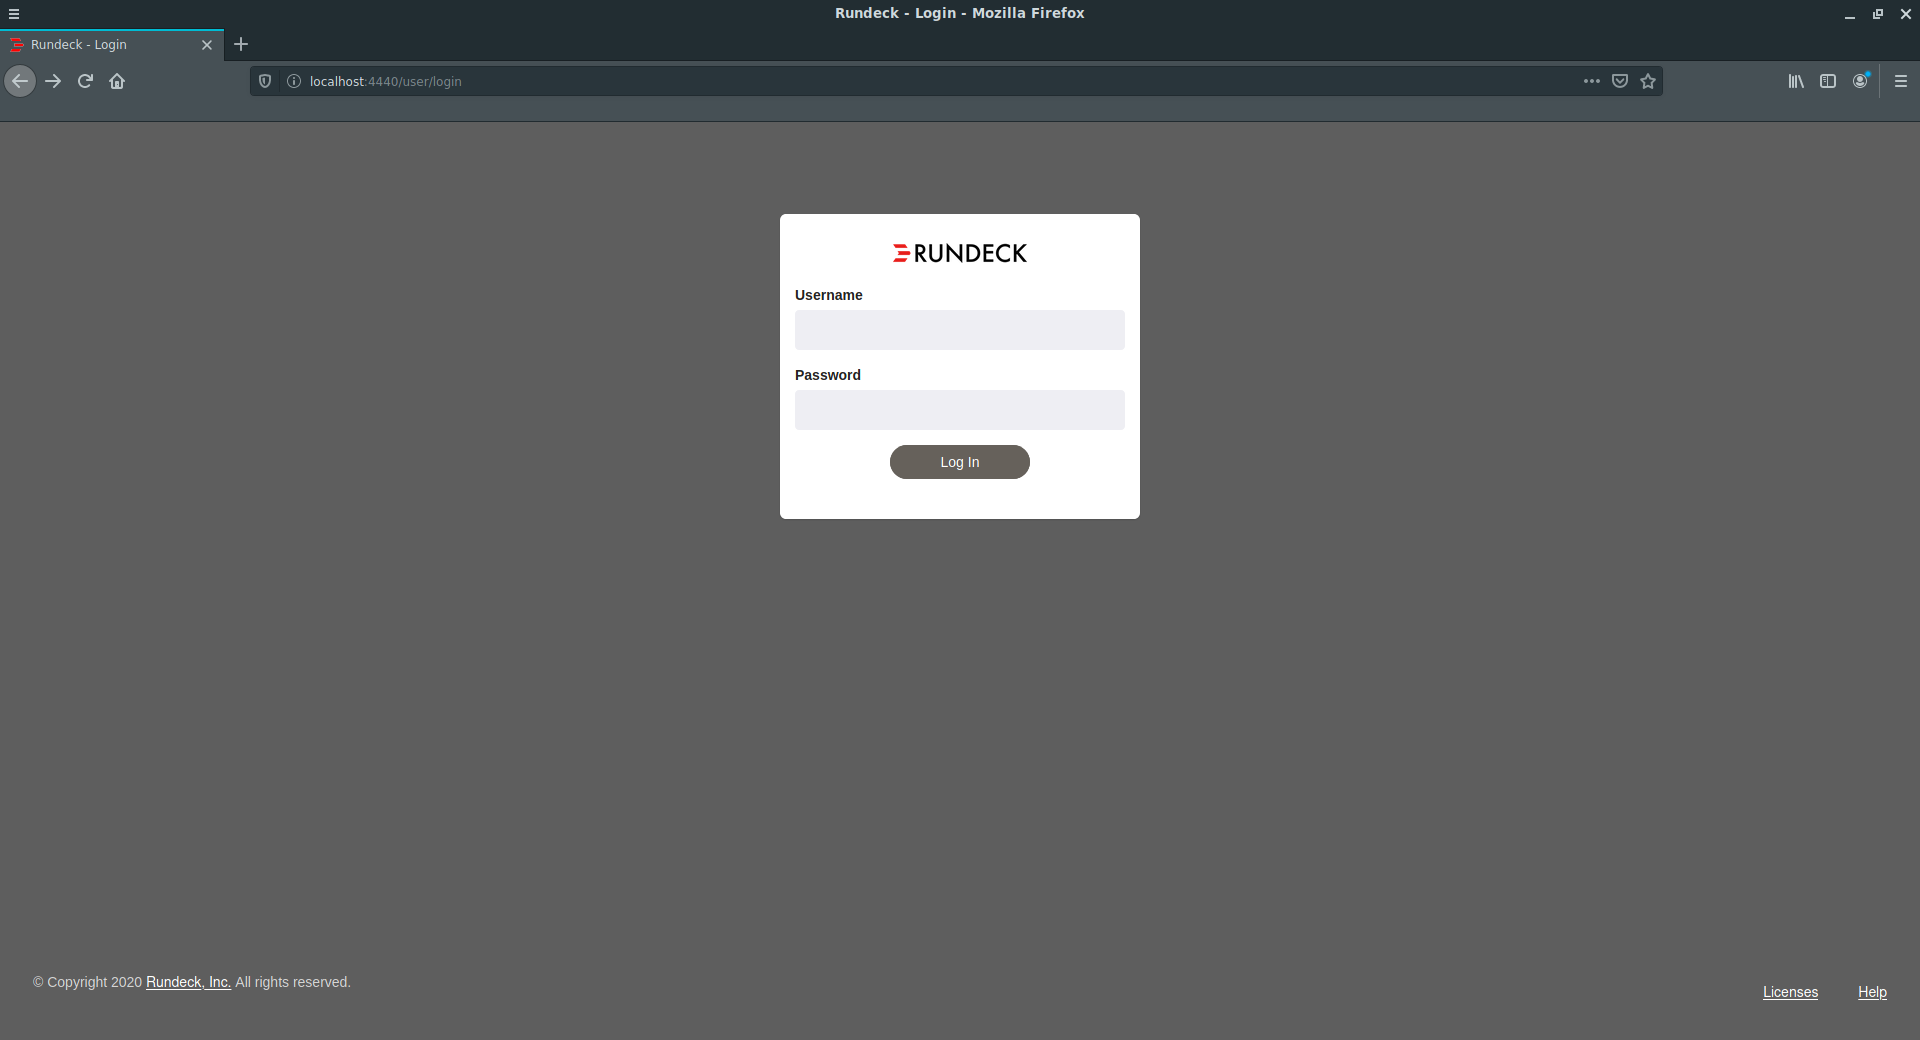
\includegraphics[scale=0.23]{images/connexion.png}
    \caption{Interface de connexion}
\end{figure}
\\
\vspace{0.5cm}
\\
\textit{Username : admin}
\\
\textit{Password : admin}

\subsubsection{Création d'un projet}
La particularité de Rundeck est de pouvoir fonctionner sous forme de projet. Cette fonctionnalité est native à Rundeck et est aussi indispensable.
\\
En effet, les projets permettent de gérer plusieurs parcs informatiques d'une même entreprise depuis une seule et unique machine.
\\
\begin{figure}[ht]
    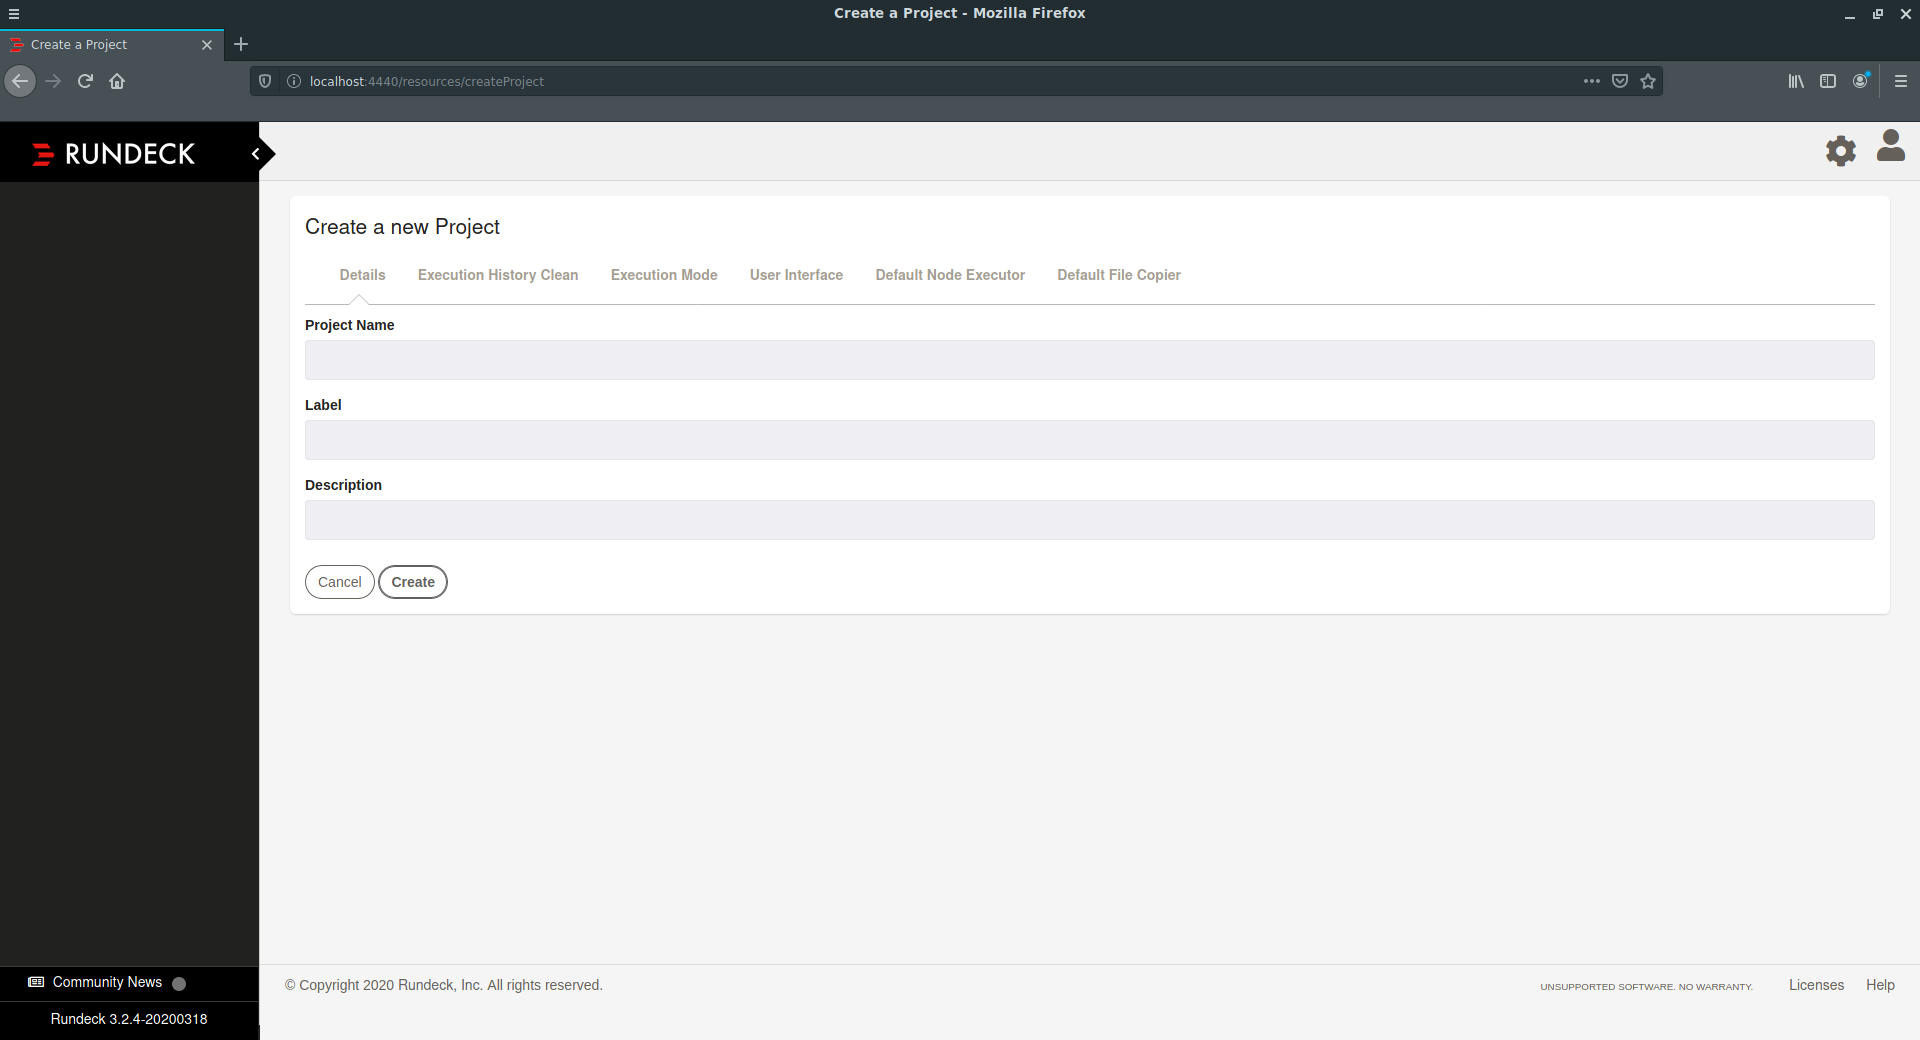
\includegraphics[scale=0.23]{images/project.png}
    \caption{Interface de connexion}
\end{figure}
\\
Lors de la création du projet, plusieurs onglets sont mis à dispositions afin de permettre une configuration complète d'un projet
\\
\begin{itemize}
    \item Les détails du jobs \textbf{"Details"}
    \item Nettoyage automatique de l'historique d'exécution \textbf{"Execution History Clean"}
    \item Paramètres d'exécution et planification \textbf{"Execution Mode"}
    \item Personnalisation de l'interface utilisateur \textbf{"User Interface"}
    \item Méthode par défaut d'exécution sur un node \textbf{"Default Node Executor"}
    \item Méthode par défaut de copie de fichier sur un node \textbf{"Default File Copier"}
\end{itemize}
\\
\vspace{0.5cm}
\\
\textbf{Informations relatives à chaque onglet :}
\\
\vspace{0.5cm}
\\
\textbf{Onglet "Details" :}
\\
L'utilisateur peut définir, depuis cet onglet, le nom ainsi qu'une courte description du projet
\\
\vspace{0.2cm}
\\
\textbf{Onglet "Execution History Clean" :}
\\
\textit{trad : Nettoyage de l'historique d'exécution}
\\
Cet onglet permet de régler le/les fréquences de nettoyage automatiques des exécutions. Ce nettoyage peut être activé ou désactivé à la demande de l'utilisateur.
\\
Des valeurs par défaut sont imposé par Rundeck telles que le nombre de jours que l'on souhaite garder l'historique (ex: Rundeck supprimera l'historique au bout de 60 jours.
\\
Rundeck propose un nombre d'exécution minimum fixé à 50 exécution, une taille maximum de l'historique limité à 500Mo ainsi que la possibilité de paramétré via \textbf{une expression de type cron}, le nettoyage automatique de l'historique.
\\
Ces valeurs sont les valeurs par défaut imposé par Rundeck mais peuvent être modifié par l'utilisateur de Rundeck.
\\
\vspace{0.2cm}
\\
\textbf{Onglet "Execution Mode" :}
\\
\textit{trad : Mode d'exécution}
\\
Cet onglet permet d'activer/désactiver l'exécution des jobs, des commandes ad-hox ainsi que la planifiaction des jobs et commandes ad-hoc.
\\
\vspace{0.2cm}
\\
\textbf{Onglet "User Interface" :}
\\
\textit{trad : Interface utilisateur}
\\
Depuis cet onglet, un README ainsi qu'un MOTD ("Message Of The Day") peuvent affiché sur certaines page lorsque qu'un utilisateur de Rundeck se connecte à l'interface
\\
\vspace{0.2cm}
\\
\textbf{Onglet "Default Node Executor" :}
\\
\textit{trad : Exécuteur de node par défaut }
\\
Par défaut, Rundeck règle l'exécuteur sur SSH, c'est-à-dire que les jobs/commandes seront exécutes via SSH. Cette méthode peut toutefois être changée si Rundeck possède des machines d'une autre distributions que Linux sous son contrôle. Rundeck propose plusieurs autres exécuteurs. Néanmoins, l'administrateur souhaite utiliser un autre exécuteur qui n'est pas présent dans la liste, ce dernier peut être télécharger via la liste des plugins (si celui se trouve à l'intérieur)  
\\
Si des clés SSH et passphrases sont stockés directement sur Rundeck, il est possible de spécifier les chemins de fichiers afin de permettre l'accès via ces protocoles
\\
\vspace{0.2cm}
\\
\textbf{Onglet "Default File Copier" :}
\\
\textit{trad : Copier de fichier par défaut}
\\
Même principe que l'onglet précèdent, celui ci permet de modifié l'utilitaire de transfert de fichiers d'une machine à une autre via Rundeck.
\\
Plusieurs méthodes sont mis à disposition par Rundeck et d'autres méthodes peuvent être téléchargées depuis la liste des plugins si la méthode demandé par l'administrateur ne se trouve pas dans la liste fournis par Rundeck
\\
Si des clés SSH et passphrases sont stockés directement sur Rundeck, il est possible de spécifier les chemins de fichiers afin de permettre l'accès via ces protocoles
\\

\subsubsection{Définition de la méthode de stockage}

Selon les choix de l'administrateur de Rundeck, plusieurs méthodes de stockages sont à disposition.

Méthode de stockage :
\begin{itemize}
    \item Base de données embarquée
    \item Base de données "personnelle"
    \item Système de fichiers
\end{itemize}

\subsubsection{Définition des nodes}
Un node permet d'ajouter un serveur, une machine que l'on souhaite automatiser avec Rundeck.
\\
Les nodes sont définis dans un fichier au format XML mais peuvent également être définis dans un fichier au format YAML et JSON. Cette définition doit suivre une syntaxe imposé par Rundeck. On peut définir autant de nodes que l'on souhaite dans ce même fichier.
\vspace{0.5cm}
\\
\textit{Ces exemples sont à titres indicatifs et sont fournis dans la documentation de Rundeck}
\vspace{0.5cm}
\\
\textbf{Syntaxe XML :}
\\
\begin{lstlisting}
<?xml version="1.0" encoding="UTF-8"?>

<project>
  <node name="localhost" 
        description="Rundeck server node" 
        tags="" 
        hostname="localhost" 
        osArch="amd64" 
        osFamily="unix" 
        osName="Linux" 
        osVersion="2.6.21.7-2.fc8xen" 
        username="rundeck"/>
</project>
\end{lstlisting}

\vspace{0.5cm}
\textbf{Syntaxe JSON :}
\\

\begin{lstlisting}
{
  "madmartigan.local": {
    "tags": "local,server",
    "osFamily": "unix",
    "username": "greg",
    "osVersion": "10.10.3",
    "osArch": "x86_64",
    "description": "Rundeck server node",
    "hostname": "madmartigan.local",
    "nodename": "madmartigan.local",
    "osName": "Mac OS X"
  },
  "test": {
    "tags": "alphabet, soup",
    "osFamily": "unix",
    "ssh-key-storage-path": "keys/testkey1.pem",
    "username": "vagrant",
    "osVersion": "10.10.3",
    "osArch": "x86_64",
    "description": "Rundeck server node",
    "hostname": "192.168.33.12",
    "nodename": "test",
    "osName": "Mac OS X"
  }
}
\end{lstlisting}

\vspace{0.5cm}
\\
\textbf{Syntaxe YAML :}
\\

\begin{lstlisting}
Venkman.local:
  description: Rundeck server node
  hostname: Venkman.local
  nodename: Venkman.local
  osArch: x86_64
  osFamily: unix
  osName: Mac OS X
  osVersion: 10.6.6
  tags: ''
  username: greg
\end{lstlisting}

\vspace{0.5cm}
Cette configuration est identique pour chaque ordinateur/serveur que l'on souhaite automatiser et peut également se faire dans plusieurs fichiers dés lors que l'on utilise une base de données. Dans notre cas, toutes les machines sont enregistrées dans un seul fichier.
\vspace{0.5cm}
\\
\textbf{Informations sur la syntaxe}
\begin{itemize}
    \item name : nom de l'ordinateur/serveur (obligatoire)
    \item description : brève description du node (facultatif)
    \item tags : nom permettant l'identification du node (facultatif)
    \item hostname : adresse IP de la machine (obligatoire)
    \item osArch : Architecture du système (facultatif)
    \item osFamily : Famille du système (facultatif)
    \item osName : Nom du système (facultatif)
    \item osVersion : Version de l'OS (facultatif)
    \item username : compte avec lequel rundeck se connecte à la machine distante (obligatoire)
\end{itemize}
\vspace{0.5cm}
La définition d'un node dans le format YAML ou JSON diffère légèrement du format XML.

\subsubsection{Clés SSH}
Rundeck requiert les clés SSH de chaque machine qu'il a sous son contrôle. Ces clés peuvent être créées et enregistrées sur les machines en prenant soins d'être connecté avec un utilisateur dédié. Ces clés peuvent également être enregistré sur la base de données de Rundeck

\subsubsection{Définition des jobs}
La définition d'un "job" est l'étape la plus importante. En effet, ce système est l'atout principal de Rundeck.
\\
Un job est décomposé en plusieurs étapes (\textit{step en anglais}). Une étape correspond à une commande ou un script
\\
Les jobs se définissent de la même manière, et ceux peut importe la manière dont Rundeck est configuré.
\\
La définition d'un job se fait sur l'interface WEB et propose plusieurs onglets de configurations :

\begin{itemize}
    \item Les détails du jobs "\textbf{Details}"
    \item L'ordre d'exécution "\textbf{Workflow}"
    \item Les noeuds "\textbf{Nodes}"
    \item La planification de l'exécution "\textbf{Schedule}"
    \item Les notifications "\textbf{Notifications}"
    \item Les options diverses "\textbf{Others}"
\end{itemize}
\\
\vspace{0.5cm}
\\
\textbf{Informations relatives à chaque onglet :}
\\
\vspace{0.5cm}
\\
\textbf{Onglet "Details" :}
\\
L'utilisateur peut définir, depuis cet onglet, le nom ainsi qu'une courte description du job
\\
\vspace{0.2cm}
\\
\textbf{Onglet "Workflow" :}
\\
\textit{trad : flux de travail}
\\
Cet onglet permet la définition de la méthode d'exécution. Cet onglet permet également de définir le/les tâches à exécuter.
\\
Rundeck propose lors du paramétrage, de continuer l'exécution du jobs même si une "step" échoue. 
\\
Rappel : une step n'est qu'une petite partie d'un job et non le job complet.
\vspace{0.5cm}
\\
\textbf{Méthodes d'exécution :}
\begin{itemize}
    \item Node First : Exécute toute les étapes d'un job sur le noeud 1, puis sur le noeud 2 etc...
    \item Parallel : Exécution de tous en parallèle et en même temps sur tous les noeuds
    \item Sequential : Le step 1 sera joué sur le noeud 1 puis noeuds 2 puis noeud X ensuite le step 2 ainsi de suite
\end{itemize}
\\
\vspace{0.2cm}
\\
\textbf{Onglet "Nodes" :}
\\
\textit{trad : Noeuds}
\\
Cet onglet permet de définir les nodes sur lequel/lesquels le job va être exécuté. Rundeck propose à l'utilisateur si le job soit être soit lancé sur la machine qui contient Rundeck, soit sur les machines que Rundeck à sous son contrôle.
\\
Beaucoup de paramètres sont disponibles tels que les filtres où l'administrateur peut décider sur quels noeuds il souhaite exécuter ce job. Cette notion implique de bien rédiger le fichier contenant les nodes.
\\
Depuis cette onglet, l'administrateur peut également dire à Rundeck que faire pour une situation donnée (ex: Si le node échoue, on peut soit arrêter complètement le job, soit continuer sur les nodes restants.
\\
\vspace{0.2cm}
\\
\textbf{Onglet "Schedule" :}
\\
\textit{trad : Planifier}
\\
Comme son nom l'indique, cet onglet permet de programmer l'heure d'exécution du job, mais il permet également de définir la fréquence d'exécution.
\\
La possibilité de planification peut être désactivé depuis cet onglet, de même pour l'exécution.
\\
Rundeck propose 2 manières de planifier un job :  De manière simple en sélectionnant l'heure et la fréquence, ou alors via une expression cron 
\\
\vspace{0.2cm}
\\
\textbf{Onglet "Notifications" :}
\\
Depuis cet onglet, peut être définit la manière dont sera notifié l'administrateur de Rundeck.
\\
Une notification peut être envoyée en cas de succès de job, d'échec, une notification au démarrage, sur des nouvelles tentatives d'exécution de jobs si celui-ci échoue une première fois.
\\
Deux méthodes de notifications sont disponibles : Webhook ou Email
\\
\textbf{Email} :  Mail contenant diverses informations telles que le job exécuter, l'heure d'exécution, son statut (réussite/échec/démarrage/nouvelle tentative), la/les machine(s) où le job à était exécuté. Toutes ces informations sont envoyés à l'administrateur de Rundeck
\\
\textbf{Webhook} : Un webhook contiendra les mêmes informations qu'un mail et se feront au travers d'un rappel HTTP. Cela peut être traduis par une notification en temps réel 
\\
\vspace{0.2cm}
\\
\textbf{Onglet "Others" :}
\\
\textit{trad : Autres/Divers}
\\
Cet onglet est essentiellement consacrés au logs et aux tentatives sur les jobs, on peut définir la nature du fichier de logs (fichier classique ou fichier pour debug) ainsi que la taille d'un fichier de logs (ex : 100 lignes par fichiers), autoriser les multiples exécution du job, le nombre de tentatives, le temps de réponses d'un job, le delais entre tentatives
\\
\section{Conclusions}

\newpage
\section{Bibliographie}

\begin{itemize}
    \item \url{https://docs.rundeck.com/docs/administration/install/}
    \item \url{https://docs.rundeck.com/docs/manual/}
    \item \url{http://docs.buildbot.net/current/index.html}
    \item \url{https://github.com/rundeck/rundeck}
    \item \url{https://docs.rundeck.com/docs/administration/configuration/config-file-reference.html}
    \item \url{https://tech.oyster.com/rundeck-vs-crontab-why-rundeck-won/}
    \item \url{https://www.edureka.co/blog/what-is-jenkins/}
\end{itemize}

\newpage
\section{Annexes}

\end{document}
